\begin{comment}
	\section*{Introducción}
	
\end{comment}

\section*{Procedimiento}
Para la práctica propuesta se tomó como base el procesador de un solo ciclo elaborado en la práctica pasada; para la primera parte de este trabajo, se inició por añadir cada uno de los registros del Pinelined con el propósito de poder almacenar y propagar las señales necesarias para cada una de las etapas; asimismo, se crearon nuevas señales como el $BranchD$ que le indica al procesador cuando la instrucción que se encuentra en la etapa de decodificación, corresponde a un salto; por otro lado, también se realizó la modificación en las $Flags$ del procesador, ya que estas solo deben actualizarse si se decodifica alguna instrucción que las altere, en caso contrario estas permanecen, por eso también se modificó la forma en la cual estas se actualizaban, pasando de ser síncronas manejadas por la señal del reloj, a ser asíncronas con muxes, que de acuerdo al $FlagWrite$ deciden cuál de las dos señales se debe mantener en las flags.\\

Es importante resaltar, que también se propagó la señal $Brl$ creada en la práctica 6 desde la unidad de control, puesto que esta era necesaria para guardar la dirección de la memoria en el registro $R14$ en la quinta etapa del procesador, con el propósito de modificar el $Pc$ una vez terminada la ejecución de la función. Además, en la primera etapa, es decir en la etapa del $Fetch$, se propagó el Pc con el fin de que este estuviese adelantado 8 posiciones con respecto a la instrucción que se estaba ejecutando, también es relevante anotar que se decidió propagar la instrucción completa hasta la etapa del $Execute$, puesto que una parte de esta era necesaria para identificar el registro al cual le correspondía almacenar el $ResultW$ en la quinta etapa del procesador, y la otra parte es utilizada para el manejo del módulo $shifter$ construido en el procesador de un solo ciclo, debido a que con esta se identifica cuál es la operación que corresponde a realizar.\\

Para concluir esta primera parte, se procedió con la implementación del $NOP$, con el fin de resolver los problemas de dependencia de datos que existen aún en este procesador debido a que aún no está construida la $Unidad de Hazards$, esta recibe la codificación $e320f000$; en este punto se debe indicar desde la unidad de control que el procesador se pare deshabilitando todas las señales que permiten la escritura en cada una de las etapas.\\

Al llegar a este punto, se decide poner a prueba al procesador mediante dos códigos, el primero de ellos realizado por el equipo de estudiantes y el segundo brindado por la guía de este trabajo. A continuación se observa cada uno de los códigos con sus respectivas simulaciones:
  
\subsubsection*{Primer código elaborado:}
\begin{lstlisting}
	.global
	_start:
	MOV 	R0, #0
	LDR 	R1, [R0, #0]
	ASR 	R2, R1, #31
	LSL 	R3, R2, #31
	LSR		R4, R2, #15
	ROR 	R5, R4, #31
	BL		Store
	End:
	B End
	Store:
	STR		R5, [R0, #4]
	MOV		PC, LR
\end{lstlisting}

\begin{figure}[H]
	\centering
	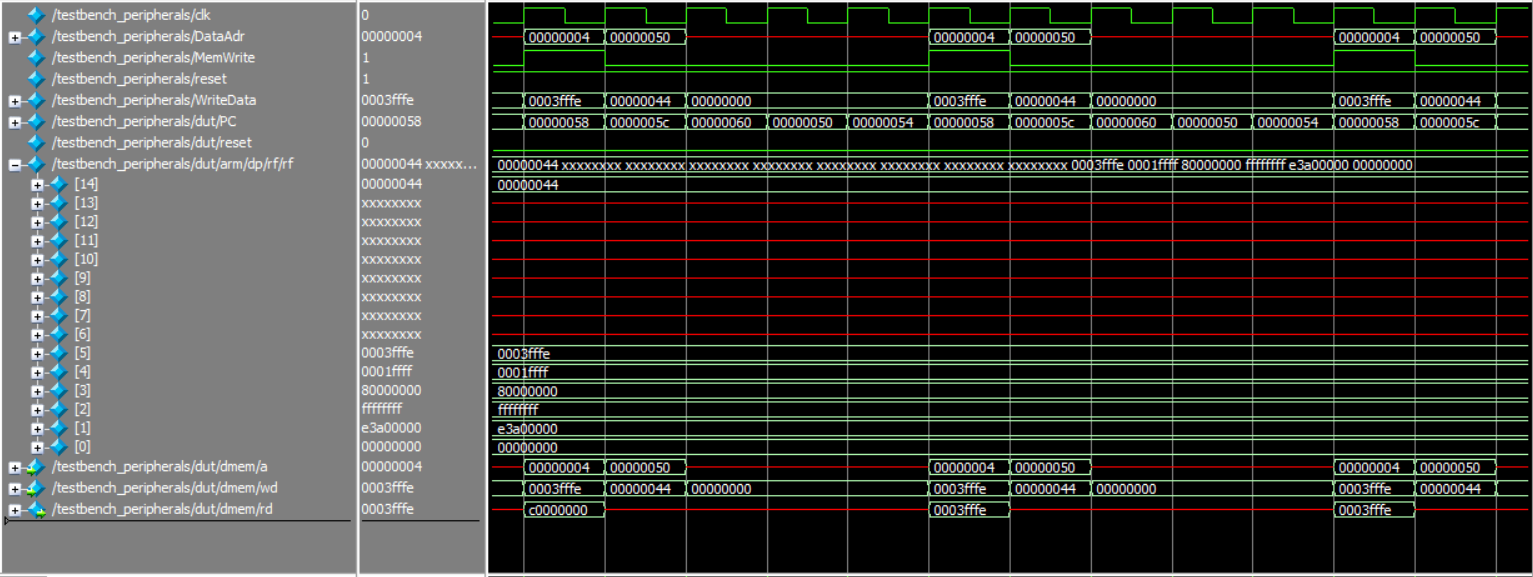
\includegraphics[width = \linewidth]{images/SimulacioncreadasinH.PNG}
	\caption{Prueba del procesador implementado con el código creado sin la Unidad de Hazards.}
	\label{fig:Código creado sin unidad de Hazards}
\end{figure}

En la memoria de datos se almacenó el valor hexadecimal $0xE3A00000$, por eso, en la figura se puede notar que los valores de los registros son los siguientes:

\begin{itemize}
	\item $R0:0x00000000$
	\item $R1:0xE3A00000$
	\item $R2:0xFFFFFFFF$
	\item $R3:0x80000000$
	\item $R4:0x0001FFFF$
	\item $R5:0x0003FFFE$
	\item $R14 o LR:0x00000044$
\end{itemize}

A esto se añade que la instrucción $STR$ escribe en la memoria el valor $R5:0x0003FFFE$ %%terminar de resolver esta pregunta
\subsubsection*{Segundo código elaborado:}
\begin{lstlisting}
	.global
	_start:
	MOV 	R0, #0
	LDR 	R1, [R0, #0]
	ASR 	R2, R1, #31
	LSL 	R3, R2, #31
	LSR	R4, R3, #15
	ROR 	R5, R4, #31
	BL		Store
	End:
	B End
	Store:
	STR		R5, [R0, #4]
	MOV		PC, LR
\end{lstlisting}

\begin{figure}[H]
	\centering
	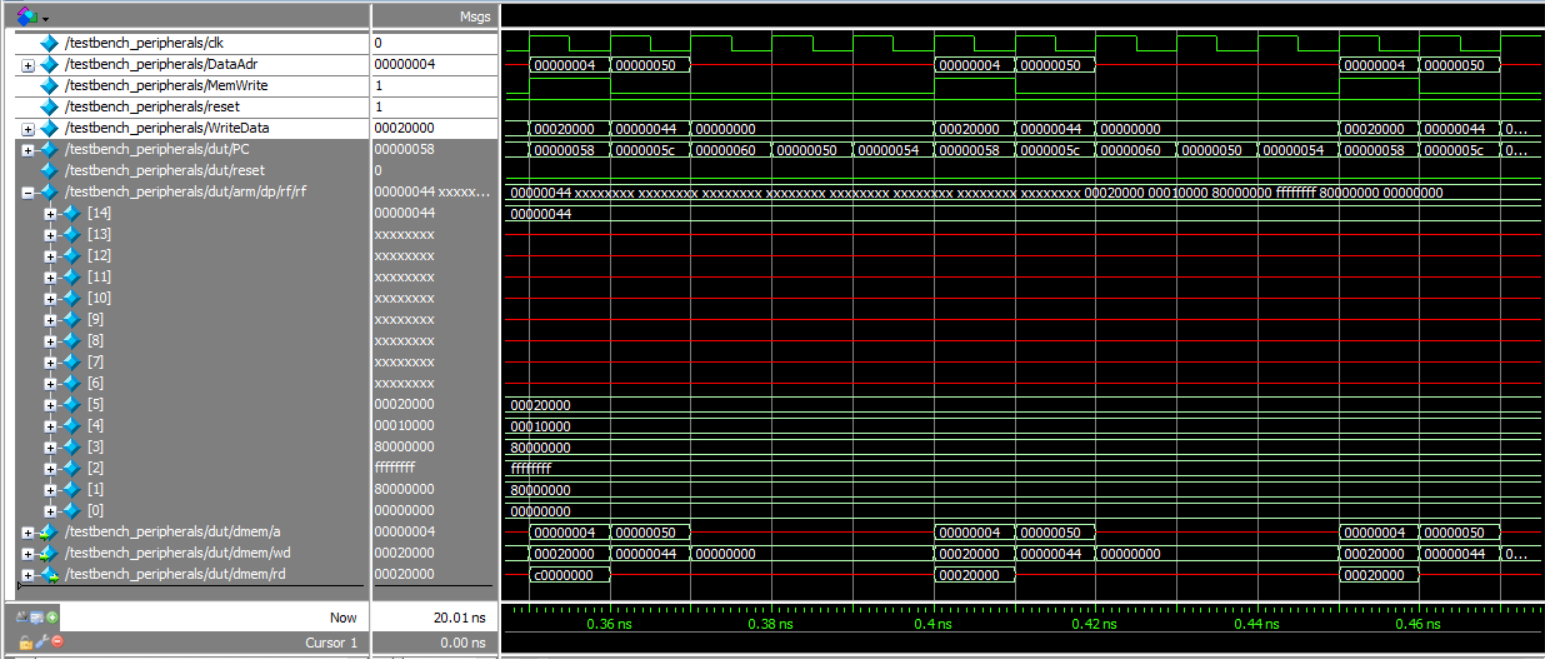
\includegraphics[width = \linewidth]{images/SimulacionGuiaSinHazards.PNG}
	\caption{Prueba del procesador implementado con el código brindado por la guía sin la Unidad de Hazards.}
	\label{fig:Código guiá sin unidad de Hazards}
\end{figure}

Seguidamente, al realizar las pruebas con el código mostrado anteriormente y con el valor hexadecimal $0x80000000$ almacenado en la memoria de datos, es posible observar que los valores de los registros son los siguientes:
\begin{itemize}
	\item $R0:0x00000000$
	\item $R1:0x80000000$
	\item $R2:0xFFFFFFFF$
	\item $R3:0x80000000$
	\item $R4:0x00010000$
	\item $R5:0x00020000$
	\item $R14 o LR:0x00000044$
\end{itemize}

A esto se añade que la instrucción $STR$ escribe en la memoria el valor $R5:0x0003FFFE$ %%terminar de resolver esta pregunta\\
Cabe anotar que se agregaron 16 $NOPs$ a la memoria de instrucciones, los cuales fueron repartidos de la siguiente manera: 2 entre cada instrucción de procesamiento de datos y carga de datos desde la memoria a uno de los registros que corresponde a las 6 líneas de código; sin embargo, a la hora de ejecutar el $Bl$ se puede ver que esta no crea una dependencia de datos con la anterior, por los que la operación $ROR$ y el comando $BL$, quedan seguidas en ejecución; después se agrega tres más, ya que $STR$ depende del valor contenido en el registro $R5$, además de que es pertinente esperar la cantidad de ciclos suficientes que permitan al procesador almacenar en memoria; finalmente, se agregan otros tres $NOPs$ seguidos del salto incondicional para que no se carguen más instrucciones en el procesador y pueda mantenerse en este ciclo. Adviértase que, al final del cifrado de las operaciones, eran necesarios otros tres $NOPs$, porque el no agregarlos trae consigo que el procesador cargue otras instrucciones inexistentes en la memoria, que hubiesen dañado la ejecución del programa; no obstante, aparentemente se cargaron $0s$ los que impedía el daño en el primer registro del $Register File$.\\

Para la segunda parte se implementa la unidad de $Hazards$ que se muestra en la imagen (referenciar), y explicada durante las sesiones de clase; esta unidad crea señales que controlan algunos registros del Pinelined, habilitando o deshabilitando el paso de los datos y realizando la limpieza de algunas de las etapas cuando es necesario, por ejemplo, cuando se decodifica una instrucción de salto y al evaluar las banderas en la etapa del $Execute$ esta se cumple, el procesador debe limpiar las operaciones cargadas en las dos etapas anteriores, mediante las señales $FlushE$ y $FlushD$ que manejan el clear de los registros; del mismo modo, este permite hacer llegar ciertos datos cuando son requeridos en el momento en el que estén listos, resolviendo así, los inconvenientes de dependencias de datos que se presentaban en el procesador desarrollado en la primera parte del presente trabajo, mejorando la eficiencia del mismo, puesto que no requiere de las 5 etapas o detenerlo durante varios ciclos para garantizar su correcto funcionamiento.\\ 

Nuevamente se carga la memoria de instrucciones que contiene el código proporcionado por la guía de manera inicial; al correr la simulación se puede notar que los registros conservan los mismos datos obtenidos en la primera parte, lo que corrobora que el procesador opera de la manera deseada puesto que, como se mencionó anteriormente, ya fueron resueltos los problemas de dependencia de datos.\\
%%Imagen de la simulación 

\begin{figure}[H]
	\centering
	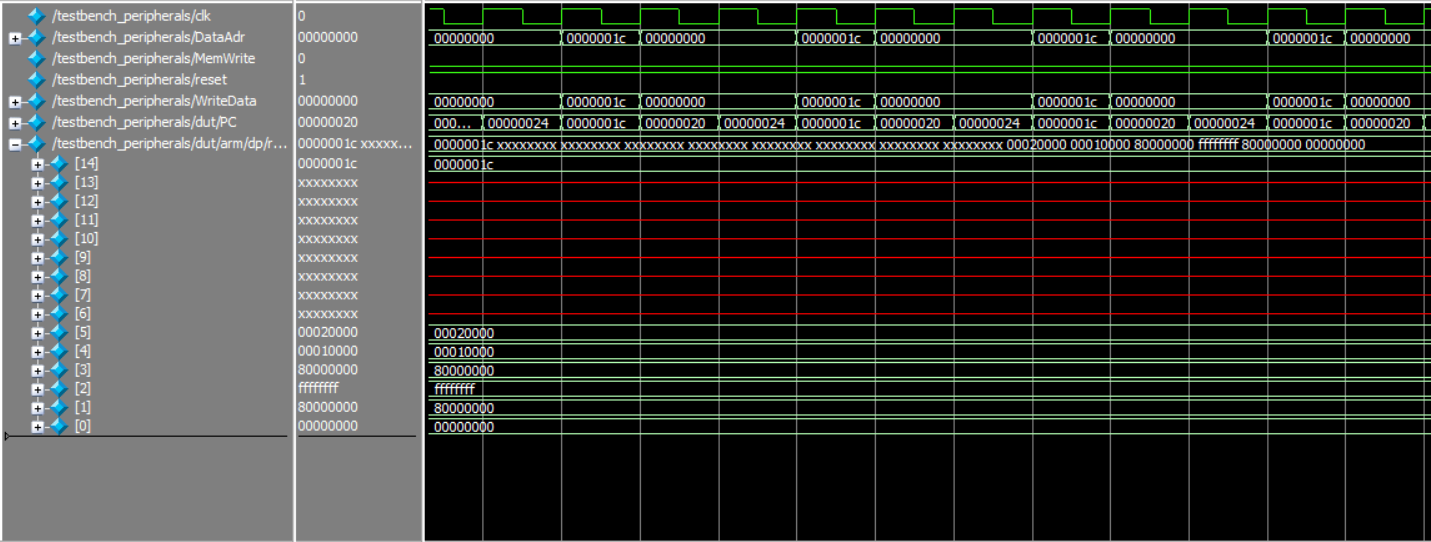
\includegraphics[width = \linewidth]{images/SGCH.PNG}
	\caption{Prueba del procesador implementado con la unidad de Hazards.}
	\label{fig:Código guiá con unidad de Hazards}
\end{figure}

Finalmente, se procede a cargar el archivo que contiene las instrucciones para la elaboración de la secuencia implementada en la practica 6, en este punto, como se aprecia en la imagen (referenciar), la señal que muestran el comportamiento de los LEDs presenta un cambio en el valor que se produce cada vez que el $Delay$ llega a 0, emulando el comportamiento de la secuencia en la tarjeta, y la variación de la misma se produce mediante la señal de $switch$ manejada desde el test bench del programa. Es necesario destacar que, se adicionó un $NOP$ en la última sección del código dentro de la función implementada, a causa de que una vez llegado a la etiqueta $DELAY$ se carga la instrucción $LDR$, habilitando la escritura en el $Register File$, pero contrariamente a escribirse de manera correcta el dato del contador en el registro, se carga el $MOV PC, LR$ por lo que se modifica el $PC$ antes de lo requerido.\\

\subsubsection*{Código de la secuencia:}
\begin{lstlisting}
	.global _start
	_start:	
	MOV R0, #0
	LDR R1, [R0,#0] //Load from switches
	LDR R1, =Switch
	LDR R2, =ROR
	LDR R5, =Time
	MOV R4, #1
	MOV R6, #0
	MOV R7, #10
	
	LOOP:
	LDR R3,[R1]
	SUBS R3, R3, #0
	LDREQ R2, [R1, #8]
	LDRNE R2, [R1, #12]
	STR R2, [R1, #4]
	
	BNE ELSE
	IF:
	ROR R2, R2, #1
	STR R2, [R1, #4]
	LDR R3,[R1]
	SUBS R3, R3, #0
	BNE LOOP
	
	BL DELAY
	
	B IF
	ELSE:
	LDR R3,[R1]
	SUBS R3, R4, R3
	BNE LOOP
	
	BL DELAY
	
	SUBS R3, R7, R6
	BNE ASR
	
	POP:
	LDREQ R2, [R1, #12]
	
	STR R2, [R1, #4]	
	MOV R6, #0
	B ELSE
	ASR:
	LSL R2,R2, #1
	STR R2, [R1, #4]
	ADD R6, R6, #1
	B ELSE
	
	
	DELAY:
	LDR R3, [R5,#0] //Counter for delay
	DLOOP:
	SUBS R3, R3, #1
	BNE DLOOP
	MOV PC, LR		
	
	
	.DATA
	Switch:		.DC.L 0x00000000
	LEDS:		.DC.L 0x00000000
	ROR: 		.DC.L 0x88888888
	Counter: 	.DC.L 0xffffffff
	Time: 		.DC.L 0x00000F00
\end{lstlisting}

\begin{figure}[H]
	\centering
	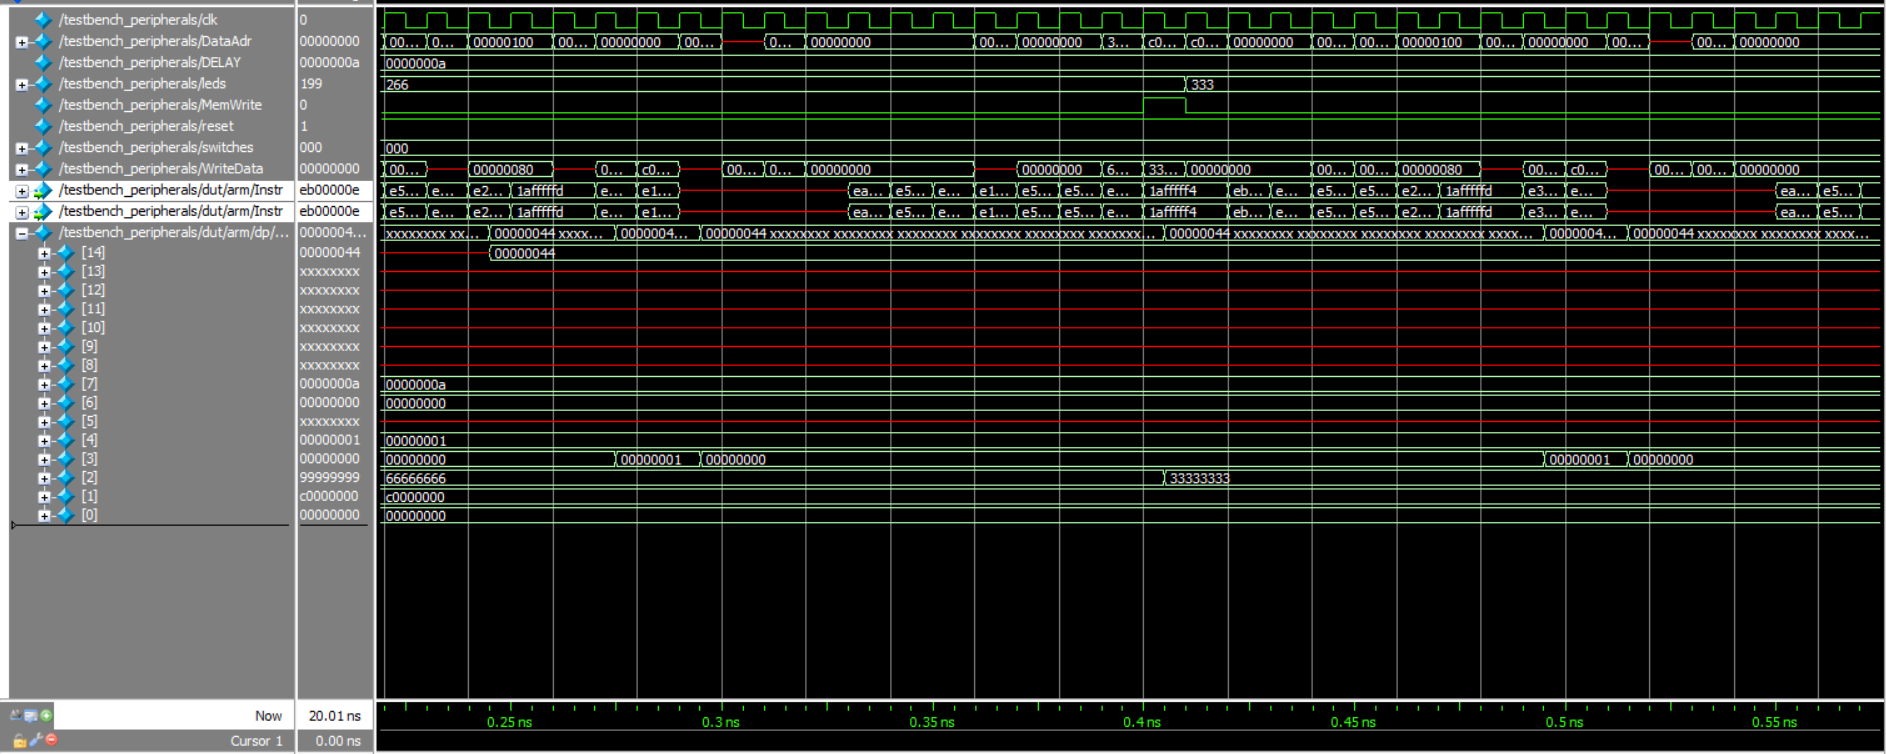
\includegraphics[width = \linewidth]{images/Switch0.PNG}
	\caption{Secuencia usando ROR.}
	\label{fig:Secuencia0}
\end{figure} 

\begin{figure}[H]
	\centering
	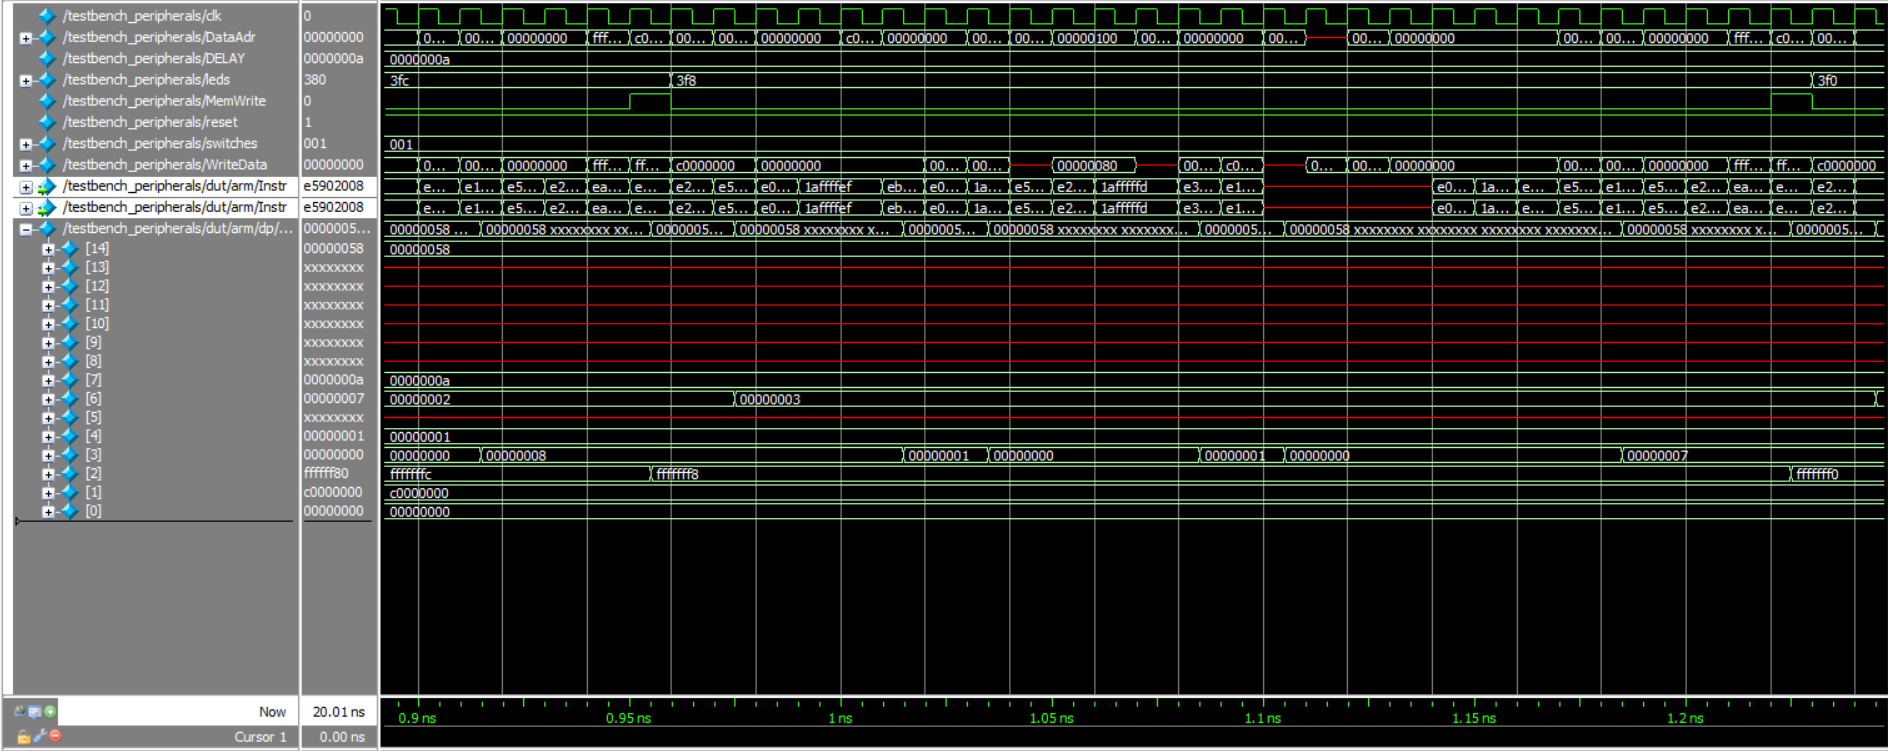
\includegraphics[width = \linewidth]{images/Switch1.PNG}
	\caption{Secuencia usando el LSL.}
	\label{fig:Secuencia1}
\end{figure} 


\section*{Conclusiones} 
Durante la presente practica se pudo apreciar la importancia que tiene recurrir a la bibliografía recomendada para el curso, porque ella contenía toda la base para la construcción del procesador, de igual modo, mencionaba aspectos fundamentales que de ser comprendidos en un principio, hubiesen simplificado la elaboración del presente trabajo; por otro lado, se debe apuntar que la elaboración de códigos más simples para poner a prueba el procesador, ayudaba a la comprobación del comportamiento del Pinelined con su respectiva unidad de Hazards, cosa que no fue tenida en cuenta durante la elaboración del mismo, costándole al equipo de trabajo múltiples retrasos demorando la culminación de la práctica, por esto fueron invertidas aproximadamente 2 horas diarias durante las últimas tres semanas.\\
A pesar de las anotaciones anteriores, puede verse que el procesador no considera un caso en cuestión, que solo fue revelado en el montaje de la secuencia, este consiste en la escritura en los registros seguido de la modificación del $PC$ en una función y la razón por la cual hacía que el procesador no tuviese la conducta esperada, fue expuesta en la parte de la explicación de la secuencia.\\



\bibliographystyle{unsrtnat}
\bibliography{docs/bibliography}